\documentclass[a4paper,12pt]{report}
\usepackage[utf8]{inputenc}
\usepackage[frenchb]{babel}
\usepackage[T1]{fontenc}
\usepackage{lmodern,textcomp}
\usepackage{graphicx}
\usepackage{listings}
\usepackage{caption}
\usepackage{fancybox}
\usepackage[pdftex]{hyperref}
\usepackage[usenames,dvipsnames]{pstricks}
\usepackage{epsfig}
\usepackage{fancyvrb}
\usepackage{alltt}

\hypersetup{%
  colorlinks= true,
  linkcolor = blue
  }
\hypersetup{
  pdftitle={Xia},
  pdfauthor={Énuma Logiciel Libre},
  pdfsubject={Xia},
  pdfkeywords={Xia, logiciel libre, html5, Inkscape}
}

\renewcommand{\thechapter}{\arabic{chapter}}
\renewcommand{\thesection}{\Roman{section}}
\renewcommand{\thesubsection}{\alph{subsection}}

% pour unifier les indications relatives aux manipulation à effectuer dans les logiciels
% à modifier au besoin
\newcommand{\chemin}[1]{\textcolor{red}{#1}}

\begin{document}
 
 % il y a, à plusieurs reprises, des paragraphes du style "<à noter"> ou "<astuces">
 % peut-être faut-il adopter le style utilisé pour ce genre de choses dans la doc se3?
 
\section{Présentation de Xia}

\subsection{Qu'est-ce que Xia?}

Xia est un logiciel libre développé par la délégation académique pour le numérique éducatif de l'académie de Versailles.
Distribué sous licence \href{http://www.gnu.org/copyleft/gpl.html}{GPLv3}, il est le successeur du logiciel «~ImagesActives~».
Xia est un convertisseur qui prend en entrée un fichier svg et fournit en sortie une image active en html5.
Au-delà des templates d'export déjà connus des utilisateurs du logiciel ImagesActives
(\href{http://images-actives.crdp-versailles.fr/spip.php?article11&lang=fr}{accordéon, boutons, etc.}),
Xia permet en outre de générer des activités interactives: jeux de glisser-déposer, discrimination, sélection, etc.

Cette documentation est un guide «~pas à pas~» pour la réalisation d'images actives.
Partant de la réalisation d'une image active simple (détourage et commentaires sans enrichissements particuliers)
elle guide l'utilisateur vers la réalisation d'images plus complexes (enrichissements multimédias, jeux, etc.)
Les exemples sont visibles en ligne (le lien est signalé en début de section), les fichiers sources (au format svg) 
sont également téléchargeables.

\subsection{Processus général}

Contrairement à ImagesActives, Xia n'intervient qu'en toute fin de processus de création de la ressource.
Comme on peut le constater sur la figure \ref{workflow_xia}, l'essentiel du travail est à effectuer
dans un logiciel de dessin vectoriel.
Nous recommandons fortement l'utilisation d'\href{http://www.inkscape.org/}{Inkscape}, logiciel libre
multi-plateforme, très aisé à prendre en main, et qui sera utilisé dans cette documentation.

\begin{figure}[htp]
 \centering
 \caption{Processus de création d'une image active avec Xia}
 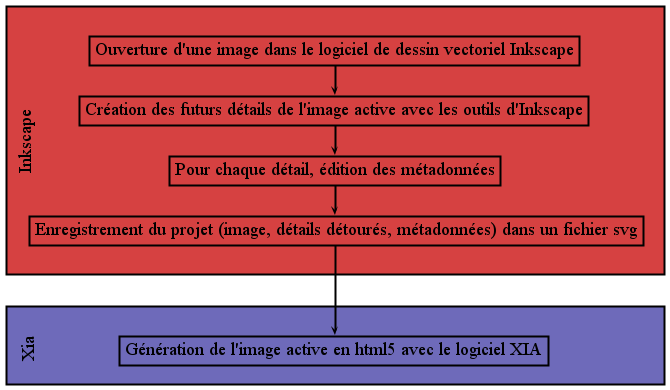
\includegraphics[width=1\textwidth]{images/workflow_xia}
 \label{workflow_xia}
\end{figure}

\section{Réalisation d'une première image active avec Inkscape et Xia: fonctionnalités de base}

\subsection{Installation d'Inkscape et de Xia}

L'installation d'Inkscape et de Xia est le seul pré-requis à la suite de la lecture de cette documentation.
Les informations nécessaires à ces manipulations se trouvent sur les sites respectifs des projets\footnote{Voir les sites d'\href{http://www.inkscape.org/}{Inkscape} et de \href{http://images-actives.crdp-versailles.fr/beta/}{Xia}.}.

\subsection{Préparation du fichier svg en vue de la génération de l'image active}\label{preparation_svg}

Les quelques manipulations décrites dans cette section sont suffisantes
pour réaliser une \href{http://geoffrey-gekiere.ac-versailles.fr/xia1}{image active «~de base~»}\footnote{Le 
\href{http://geoffrey-gekiere.ac-versailles.fr/xia1/svg/xia1.svg}{fichier svg correspondant est téléchargeable}.}, 
ayant les caractéristiques suivantes:
\begin{itemize}
 \item Détails zoomables
 \item Commentaires des détails constitués uniquement de texte non mis en forme
\end{itemize}


Une fois l'image à travailler choisie, on l'ouvre dans Inkscape (menu \chemin{Fichier} puis \chemin{Ouvrir}).
À la question posée par le logiciel («~\chemin{Lier ou incorporer l'image}~»), on choisira «~\chemin{Incorporer}~».

Parmi les nombreuses informations que l'on peut renseigner en accédant à la fenêtre de dialogue des 
\chemin{Métadonnées du document} (menu \chemin{Fichier}), trois seront prises en compte dans l'image active
une fois générée: le titre, le créateur, les droits.
Il est donc fortement recommandé de les renseigner.
Dans l'exemple suivant (voir figure \ref{titre_ia}), on voit l'importance d'un titre correctement
renseigné dans les métadonnées: il s'agit en réalité du titre de l'image active\footnote{Les champs 
«~auteur~» et «~droits~» apparaissent pour leur part dans la fenêtre «~À propos~», symbolisé par 
un bouton clicable en forme de lettre «~i~».}.

\begin{figure}[htp]
 \centering
 \caption{Le titre renseigné dans les métadonnées du document apparaît au-dessus de l'image active 
 et donne son nom à la page web de celle-ci}
 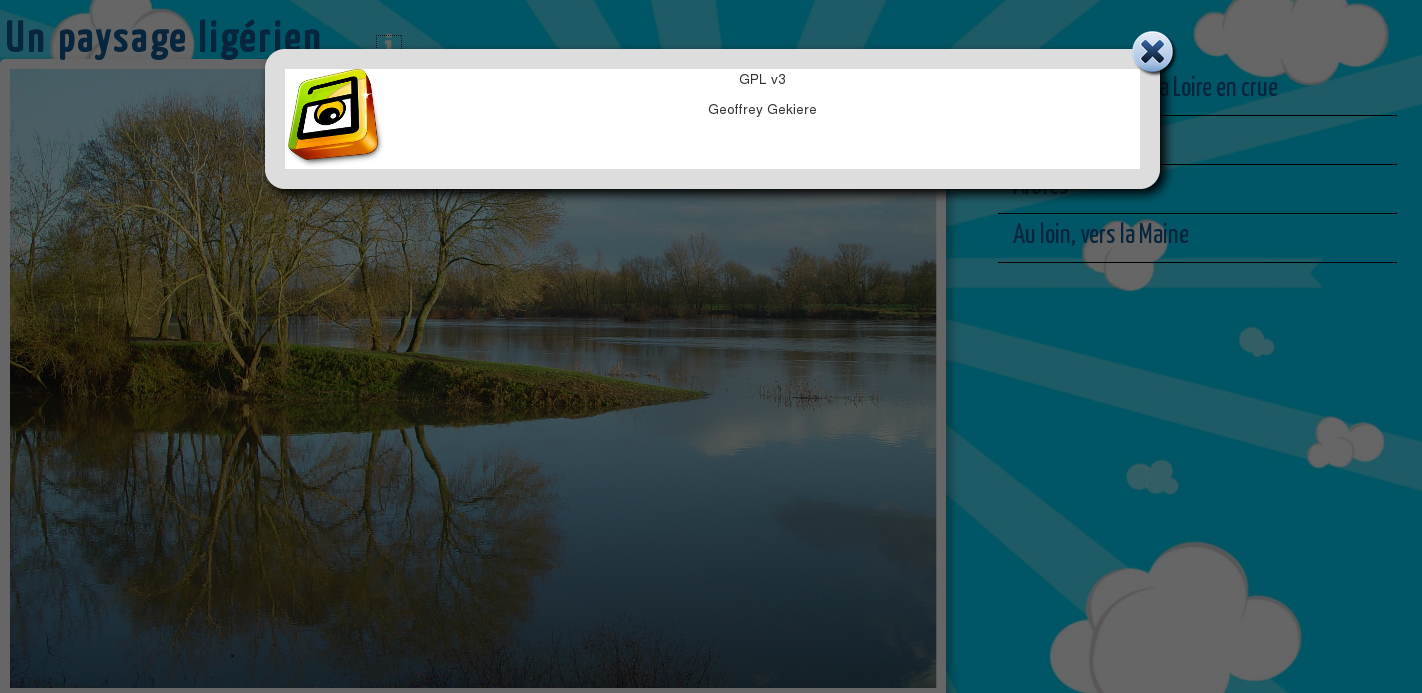
\includegraphics[width=0.7\textwidth]{images/titre_ia}
 \label{titre_ia}
\end{figure}

On peut enregistrer l'image au format svg dès le début du travail, en
passant par le menu \chemin{Fichier} puis \chemin{Enregistrer sous...}.
Pour davantage de lisibilité, on supprimera l'extension actuelle de l'image dans le champs \chemin{Nom} 
 de la fenêtre de dialogue. Enfin, dans le menu déroulant permettant de choisir le format de 
 fichier: format \chemin{SVG Inkscape (*.svg)}.

Plusieurs outils d'Inkscape sont utilisables pour détourer les détails qui deviendront actifs dans l'image générée 
par Xia. Parmi ceux-ci:
\begin{itemize}
 \item 
\includegraphics[scale=0.5]{./images/rec_carre} L'outil \chemin{Créer des rectangles et des carrés}
 \item 
\includegraphics[scale=0.5]{./images/cercles} L'outil \chemin{Créer des cercles, des ellipses et des arcs}
 \item 
\includegraphics[scale=0.5]{./images/lignes} L'outil \chemin{Dessiner des lignes à main levée}
 \item 
\includegraphics[scale=0.5]{./images/bezier} L'outil \chemin{Tracer des courbes de Bézier et des segments de droite}
\end{itemize}

% dans ce paragraphe, peut-être insérer une bidouille quelconque pour que l'allusion aux touches
% Ctrl et Maj soit plus claire (dessiner une touche de clavier?)
Sans rentrer dans le détail du fonctionnement de ces outils\footnote{Pour cela, 
se référer au \href{http://inkscape.org/doc/shapes/tutorial-shapes.fr.html}{manuel d'Inkscape}.}, on notera cependant que
les outils «~\chemin{Créer des rectangles et des carrés}~» et «~\chemin{Créer des cercles, des ellipses et des arcs}~»
 peuvent se manipuler uniquement à la souris ou en lien avec le clavier: en appuyant sur la touche Ctrl, on 
 dessine un carré, rectangle ou cercle de rapport de dimensions entier (2:1, 3:1, etc.),
 et en appuyant sur la touche Maj, on dessine autour du point de départ.

L'outil «~\chemin{Tracer des courbes de Bézier et des segments de droite}~» permet de détourer «~clic par clic~»
(on appelle les points de construction des «~nœuds~»).
On referme la figure en cliquant sur le nœud de départ.
L'outil «~courbe de bézier~» est appelé en gardant le clic de souris appuyé après avoir créé un nœud, 
puis en déplaçant le pointeur pour faire apparaitre les poignées de contrôle permettant de modeler
le segment de courbe à volonté.

À noter:
\begin{itemize}
 \item si l'utilisateur définit dans Inkscape une forme laissée ouverte (par exemple: une ligne),
Xia la «~refermera~» automatiquement en reliant par une droite le début et la fin de celle-ci.
 \item l'ordre de création des détails correspond dans l'image générée à l'ordre d'affichage des détails
 (par exemple, le détail créé en premier dans Inkscape apparaîtra en haut dans l'image active)
\end{itemize}

Une fois un détail détouré, on le sélectionne avec l'outil 
\includegraphics[scale=0.5]{./images/selection}
\chemin{Sélectionner et transformer des objets} afin de le redimensionner, le déplacer, etc.

C'est par un clic droit sur le détail détouré que l'on accède aux \chemin{Propriétés de l'objet} (voir figure \ref{proprietes_objet}),
et ainsi à la fenêtre de dialogue dans laquelle on renseigne le texte qui sera associé au détail dans l'image active
une fois générée.

\begin{figure}[htp]
 \centering
 \caption{Accès aux «~Propriétés de l'objet~», permettant de renseigner le texte 
 qui servira de commentaire au détail dans l'image active générée}
 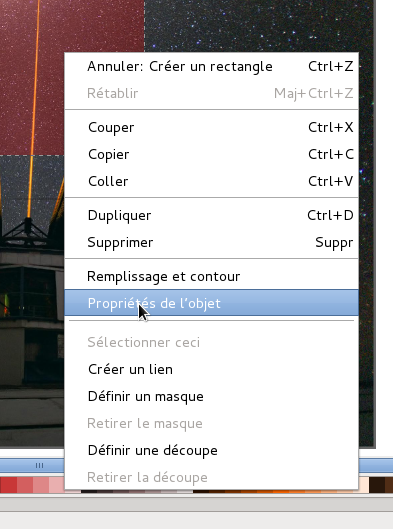
\includegraphics[width=0.3\textwidth]{./images/proprietes_objet}
 \label{proprietes_objet}
\end{figure}

Les deux champs à renseigner dans cette fenêtre sont \chemin{Titre} et \chemin{Description}.
Le titre renseigné ici sera celui du détail, la description en sera son commentaire.

Le processus décrit ci-dessus doit également être réalisé avec l'image de fond: le titre et la description renseignées
serviront d'introduction à l'image active (titre et commentaire non reliée à un détail particulier).

\subsection{Génération de l'image active dans Xia}

Quand tous les détails sont détourés et leurs métadonnées renseignées, on peut lancer le logiciel Xia.
La première icône, en haut à gauche, permet de choisir le fichier svg à générer:
\begin{center}

\includegraphics[scale=0.4]{./images/xia_open} 
\end{center}

Un clic sur l'une des icônes d'export génère une série de fichiers, dont un index.html. 
Attention: ce fichier seul est inexploitable. Tous les autres fichiers et répertoires générés lors de l'export 
sont indispensables au bon fonctionnement de l'animation. \textbf{Il est donc indispensable de dédier un répertoire 
spécifique à chaque image exportée, afin d'éviter des déconvenues}.
Il suffit d'ouvrir le fichier index.html dans un navigateur pour voir apparaître l'image active.

Les templates d'images actives «~simples~» sont les suivants:
% pertinence d'ajouter une 4e colonne pour décrire brièvement les caractéristiques de chaque export?
\begin{center}
\begin{tabular}{|l|c|c|}
\hline
Nom du thème & Icône & Exemple\\
\hline
accordionBlack\  & 
\includegraphics[scale=0.5]{./images/accordionBlack} & 
\href{http://geoffrey-gekiere.ac-versailles.fr/xia1/accordionBlack}{Paysage ligérien, export accordionBlack}\\
\hline
accordionCloud &  
\includegraphics[scale=0.5]{./images/accordionCloud} & 
\href{http://geoffrey-gekiere.ac-versailles.fr/xia1/accordionCloud}{Paysage ligérien, export accordionCloud}\\
\hline
buttonBlue &  
\includegraphics[scale=0.5]{./images/buttonBlue} & 
\href{http://geoffrey-gekiere.ac-versailles.fr/xia1/buttonBlue}{Paysage ligérien, export buttonBlue}\\
\hline
popBlue &  
\includegraphics[scale=0.5]{./images/popBlue} & 
\href{http://geoffrey-gekiere.ac-versailles.fr/xia1/popBlue}{Paysage ligérien, export popBlue}\\
\hline
popYellow &  
\includegraphics[scale=0.5]{./images/popYellow} & 
\href{http://geoffrey-gekiere.ac-versailles.fr/xia1/popYellow}{Paysage ligérien, export popYellow}\\
\hline
\end{tabular}
\end{center}

\section{Image active enrichie}

Dans cette section, nous réalisons toujours une image active classique (un détail = un commentaire),
mais nous enrichissons le contenu de celle-ci par divers moyens, comme une mise en forme avancée du texte ou des contenus 
multimédias directement insérés dans les commentaires.

L'image illustrant les manipulations décrites dans cette section est \href{http://geoffrey-gekiere.ac-versailles.fr/xia2/}
{visible en ligne}, et le \href{http://geoffrey-gekiere.ac-versailles.fr/xia2/svg/xia2.svg}{svg créé dans Inkscape est téléchargeable}.

\subsection{Mise en forme du texte}

Pour mettre en forme le texte des commentaires, on insérera les balises suivantes:

% problème d'alignement du contenu des cellules sur les lignes "<liste de puces"> et "<tracer une ligne">
\begin{center}
 \begin{tabular}{|l|l|}
 \hline
  Balises & Résultat\\
  \hline
  \hline
  ***gras*** & \textbf{gras}\\
  \hline
  **italique** & \textit{italique}\\
  \hline
  [http://dane.ac-versailles.fr Le site de la Dane] & \href{http://dane.ac-versailles/fr}{Le site de la Dane}\\
  \hline
  \{\{\{Texte brut\}\}\} & 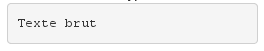
\includegraphics[scale=0.7]{./images/texte_brut}\\
  \hline
  ~* une liste\\
  ~* de puces\\
  ~~* sur 2\\
  ~~* niveaux\\ & 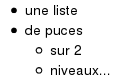
\includegraphics[scale=0.7]{./images/liste_puce}\\
  \hline
  tracer\\
  \verb|----|\\
  une ligne\\ & 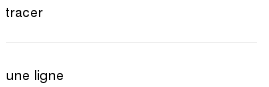
\includegraphics[scale=0.7]{./images/ligne_commentaire}
  \end{tabular}
\end{center}

\subsection{Enrichissement multimédia des détails}

L'insertion de contenus multimédias dans les commentaires des détails est extrêmement aisé:
il suffit à l'utilisateur d'indiquer l'url (relative ou absolue) de la ressource, ou d'insérer le code iframe
fourni par le service hébergeant le contenu (par exemple, la \href{https://scolawebtv.crdp-versailles.fr/}{Scolawebtv}).

Nativement, Xia génère un lecteur multimédia dans le commentaire à partir du moment où la ressource (image, son ou vidéo)
correspond à un des formats suivants:
\begin{description}
 \item [Images] jpg, jpeg, png, gif
 \item [Son] ogg, mp3
 \item [Vidéo] ogv, webm, mp4
\end{description}

Il suffira donc d'indiquer le lien relatif ou absolu vers la ressource pour que le lecteur apparaisse une fois l'image générée:
\begin{description}
 \item [Lien absolu] Si la ressource se trouve à l'adresse\\
 \verb|http://web.crdp.ac-versailles.fr/proftv/5/4/6/02546.ogg|\\
 il suffira d'indiquer cette adresse dans le champs description des propriétés de l'objet, dans Inkscape
 \item [Lien relatif] Si la ressource se trouve dans le dossier d'export ou dans un dossier situé dans le dossier d'export, on en indiquera
 l'emplacement en considérant le dossier d'export comme la racine
 (par exemple, si \verb|video.ogv| se trouve dans un répertoire \verb|videos| lui-même situé dans le dossier d'export, on indiquera dans
 le commentaire \verb|videos/video.ogv| pour que le lecteur soit créé)
\end{description}

Pour que la lecture de la ressource commence automatiquement, l'ajout de l'argument \verb|autostart| 
après l'url de la ressource est requis:\\
\verb|http://web.crdp.ac-versailles.fr/proftv/5/4/6/02546.ogg autostart|.

Les différents formats vidéos gérés par Xia ne sont pas nativement reconnus par tous les navigateurs.
Une méthode pour contourner ce problème peut consister à exporter dans les trois formats la ressource,
et à déposer les trois fichiers ainsi obtenus dans un répertoire identique, avec le même nom (seule l'extension
en .ogv, .mp4 et .webm les différencie alors):\\

% je pense qu'il y a moyen de faire vachement plus joli pour représenter l'arborescence
 % po4a: environment tikzpicture {} 
\begin{tikzpicture}
\end{tikzpicture}
 % po4a: environment alltt {} 
\parbox{0.40\textwidth}
{
\begin{alltt}
 -\textcolor{blue}{repertoire\_export}\\
 ---index.html\\
 ---[ensemble des fichiers et répertoires générés par Xia]\\
 ---\textcolor{blue}{repertoire\_videos}\\
 -----video.mp4\\
 -----video.ogv\\
 -----video.webm\\
\end{alltt}
}
\fbox{\begin{minipage}{0.50\textwidth}
	Dans l'exemple ci-contre, les répertoires, en bleu, ont été créés par l'utilisateur. 
	Dans le répertoire \textcolor{blue}{repertoire\_export}
	se trouvent les répertoires et fichiers générés par Xia, dont le fichier index.html.
	On crée également dans ce répertoire un répertoire \textcolor{blue}{repertoire\_videos} qui a pour fonction
	de stocker les vidéos qui seront appelées dans les commentaires de l'image active grâce à un lien relatif.
      \end{minipage}}


Ainsi, même si un format particulier est indiqué dans la description (en suivant l'exemple précédent: \verb|repertoire_videos/video.ogv|),
si le navigateur ne parvient pas à lire la ressource, il tentera automatiquement de lire les fichiers du même nom 
possèdant une extension différente (soit, ici, \verb|video.mp4| puis \verb|video.webm|).

Enfin, la dernière possibilité consiste à insérer dans le commentaire le code iframe d'un service d'hébergement de ressources.
Celui-ci sera interprêté et le lecteur du service s'affichera dans le commentaire, donnant accès à la ressource.

\subsection{Insertion d'images dans l'image active}\label{insertion_images}

On peut ajouter à l'image active des images (logo, puces, etc.) au format png.
Pour ce faire, dans Inkscape, retourner dans le menu \chemin{Fichier}, et choisir \chemin{Importer}
afin d'incorporer votre nouvelle image.

Cette nouvelle image ne sera visible automatiquement dans l'image active générée
que si on lui applique un fond blanc (après l'avoir sélectionnée, on choisit cette couleur dans la palette
horizontale située en bas de l'interface d'Inkscape (voir figure \ref{remplissage_blanc}).

\begin{figure}[htp]
 \centering
 \caption{Dans Inkscape, on sélectionne le png incorporé puis on lui applique un fond blanc en sélectionnant 
 cette couleur dans la palette horizontale afin de le rendre visible automatiquement}
 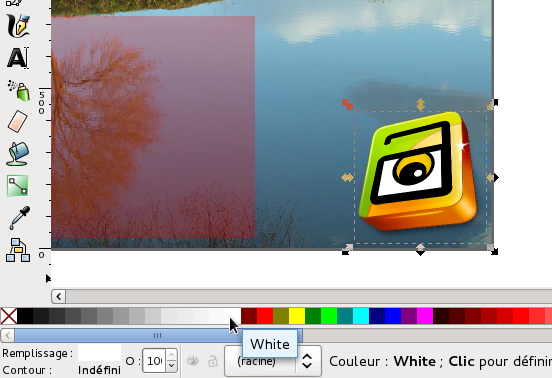
\includegraphics[width=0.6\textwidth]{images/remplissage_blanc}
 \label{remplissage_blanc}
\end{figure}

En indiquant une url dans le champs \chemin{Titre} des \chemin{Propriétés de l'objet}, l'image incorporée
devient une icône clicable renvoyant vers la page web en question.

\subsection{Afficher une question et accéder à une réponse}

Pour insérer dans un détail un bouton «~\textit{Réponse}~» clicable bloquant momentanément l'accès à la suite du commentaire,
rien de plus simple!

Il suffit en effet d'insérer dans la description, à l'endroit souhaité, la ligne\\
\verb|Réponse:| ou \verb|réponse:| et de rédiger en-dessous le texte que l'on souhaite voir apparaître.

\subsection{Contrôler le comportement des détails: affichage immédiat et désactivation
de l'effet «~zoom~»}

Par défaut, le comportement d'un détail dans l'image active générée est le suivant:
\begin{itemize}
 \item Le détail ne se révêle qu'au survol de la souris ou qu'à la sélection du titre du commentaire
 qui lui est associé
 \item Un second clic sur un détail déjà sélectionné effectue un zoom sur celui-ci
\end{itemize}

Ces deux comportements sont modifiables par l'application, dans Inkscape, d'un fond de couleur blanche ou noire
aux détails détourés (voir section \ref{insertion_images} et figure \ref{remplissage_blanc}):
\begin{description}
 \item [Détail auquel est appliqué un fond de couleur blanche] Une fois l'image générée, 
 le détail sera immédiatement visible, sous la forme d'un aplat de couleur opaque (masquant
 logiquement l'image de fond). Une fois sélectionnée, l'image de fond est révêlée et le détail demeure zoomable
 \item [Détail auquel est appliqué un fond de couleur noire] Le détail n'est visible qu'en étant sélectionné, mais
 n'est pas zoomable.
\end{description}

Conséquence logique: un détail ne pouvant se voir appliquer à la fois un fond blanc et noir, il ne peut être à la
fois immédiatement visible \textit{et} non-zoomable.

À noter: Xia ne prend pas en compte le degré d'opacité du fond appliqué au détail, mais uniquement la couleur.

\subsection{Contrôler l'ordre d'affichage des détails dans l'image active}

% à rédiger

\section{De l'interactivité à l'activité: réaliser des jeux avec Xia}

Jusqu'à présent, cette documentation a uniquement abordé la réalisation d'images actives au sens «~traditionnel~»:
une image de fond dont des détails détourés sont associés à des commentaires plus ou moins enrichis.

Ce type d'image permet de mettre en œuvre des scénarios pédagogiques ne manquant pas d'intérêt 
(découverte progressive de documents, fabrication collaborative par les élèves d'images actives), 
mais Xia va beaucoup plus loin en permettant la réalisation de jeux et d'activités variées, dans lesquelles
l'utilisateur est amené à réaliser infiniment plus d'actions que de simples clics sur des détails ou des commentaires.

\subsection{Premier principe ludique: sélectionner, retrouver dans l'image}

\textit{Le principe ludique est le suivant: on propose une image dans laquelle l'utilisateur 
doit sélectionner un certain nombre de détails en fonction d'une consigne. 
La réalisation de l'objectif énoncé déclenche l'affichage d'un message.}

C'est en réalité l'activité, voire l'image active la plus simple à réaliser. Il suffit en effet 
au créateur de la ressource de détourer les éléments que l'utilisateur doit retrouver.

La consigne à destination de l'utilisateur de l'image active est à renseigner 
dans les métadonnées du document. En effet, au moment de l'export, Xia cherche les informations
situées dans le champs \chemin{Description} des métadonnées du document 
(voir section \ref{preparation_svg} et figure \ref{titre_ia}), afin d'en faire une «~pop up~»
qui s'affichera lors de l'ouverture de l'image générée. L'utilisateur lit alors la consigne et ferme
la pop up pour jouer.

L'utilisateur de la ressource a donc pour objectif de cliquer sur un certain nombre de détails.
Une fois un certain nombre de ces détails repérés et cliqués, un message informant de la réussite de l'exercice
apparaît. Celui-ci est créé dans la \chemin{Description} des \chemin{Propriétés de l'objet} de l'image de fond
\footnote{Quand une image active «~traditionnelle~» est générée, cette manipulation
permet la création du commentaire introductif à l'image, non relié à un détail particulier
(voir section \ref{preparation_svg}).}. 
Deux informations sont nécessaires pour que ce message apparaisse:
le nombre de bonnes réponses déclenchant le message\footnote{Ce nombre est à la discrétion
du créateur de la ressource et peut tout à fait être inférieur au nombre total de détails placés sur l'image},
et le message en lui-même. Ce tableau résume les balises à insérer:

% le multicolumn refuse le \verb... à corriger
\begin{center}
 \begin{tabular}{|l|p{2in}|p{2in}|}
 % \hline
% \multicolumn{3}{|c|}{Informations à renseigner dans le champs Description des Propriétés de l'objet}\\
 \hline
  Objectif & Renseigner le nombre de bonnes réponses & Afficher un message\\
  \hline
  Balise & \verb|<score></score>| & \verb|<message></message>|\\
  \hline
  Exemple & \multicolumn{2}{|l|}{<score>6</score>}\\
   & \multicolumn{2}{|l|}{<message>Bravo, vous avez réussi à classer}\\
    & \multicolumn{2}{|l|}{correctement tous les éléments</message>}\\
  \hline
 \end{tabular}
\end{center}

Astuce: les balises \verb|<message></message>| n'empêchent en rien l'enrichissement du message. 
On peut imaginer de proposer le visionnage d'une image, d'une vidéo, ou l'affichage d'un lien vers un second exercice, afin 
de «~chaîner~» les activités par degré de difficultés.

Enfin, la génération d'une l'image active ayant pour principe ludique la sélection de détails
correspond dans Xia à l'export \chemin{game1clic}:

\begin{center}

\includegraphics[scale=0.7]{./images/game1clic} 
\end{center}


\subsection{Second principe ludique: classer, légender, hiérarchiser}

\textit{Second principe ludique: une image de fond contient des étiquettes qu'il faut déplacer et 
déposer sur les bons détails. Lorsque tous les éléments ont été remis à leur place, un message 
confirme la résolution du jeu.}

La démarche pour la réalisation d'un jeu de ce type est la suivante:
\begin{enumerate}
 \item Dans Inkscape:
\begin{itemize}
 \item Choisir une image de fond
 \item Préparer les «~étiquettes~» à déplacer (de petites images au format png), 
 et les importer dans Inkscape
 \item Faire correspondre chaque étiquette à sa zone de dépôt (en réalité, un détail détouré)
 grâce aux métadonnées renseignées
\end{itemize}
 \item Dans Xia
 \begin{enumerate}
  \item Générer le svg ainsi préparé avec le thème «~gameDragAndDrop~»
 \end{enumerate}
\end{enumerate}

Une fois les «~étiquettes~» créées (un moyen simple est d'utiliser un utilitaire de capture d'écran 
capable de produire des images au format png) et importées dans Inkscape, il s'agit de les faire 
correspondre aux détails censés les accueillir\footnote{Une étiquette ne peut correspondre qu'à un détail.}.

Le tableau suivant résume les métadonnées à renseigner dans les \chemin{Propriétés de l'objet}
dans l'étiquette et le détail correspondant:

\begin{center}
\begin{tabular}{|p{1.in}|p{2.5in}|p{1.5in}|}
\hline
 & Étiquette (objet à déplacer) & Détail détouré (réceptacle de l'étiquette)\\
\hline
Champs ID & \textit{Laisser l'ID créé par Inkscape} & \verb|Titre_Detail|\\
\hline
Champs Description & \verb|<target>Titre_Detail</target>| & \textit{Laisser ce champs vide}\\
\hline
Champs Interactivité > Onclick & \textit{Laisser ce champs vide}& \verb|off|\\
\hline
\end{tabular}
\end{center}

Pour résumer, le créateur de la ressource fait savoir à Xia quelle étiquette correspond à quel détail en faisant 
correspondre le champs \chemin{ID} du détail (réceptacle) au champs \chemin{Description} de l'étiquette 
(objet à déplacer). La seule subtilité consiste à entourer, dans le champs \chemin{Description}
de l'étiquette, l'ID correspondante d'une balise \verb|<target>| et \verb|</target>|.

Une astuce: si l'image active contient de nombreux détails réceptacles de taille identique, 
il est recommandé d'en créer une, de lui appliquer la caractéristique \chemin{Interactivité > OnClick} = \verb|off|, 
puis de copier-coller ce détail autant de fois que nécessaire. Conservant cette option, 
le créateur de la ressource n'aura pas besoin d'aller l'appliquer à chaque détail créé.

La génération d'une l'image active ayant pour principe ludique le glisser déposer 
correspond dans Xia à l'export \chemin{gameDragAndDrop}:

\begin{center}

\includegraphics[scale=0.7]{./images/gameDragAndDrop} 
\end{center}

\subsection{Enrichir ses jeux: quelques astuces...}

Ajouter un son lors de l'action d'un utilisateur.
Montrer à l'utilisateur sa progression lors de l'utilisation d'un jeu game1clic.
Ajouter un effet «~magnétisme~» dans le jeu gameDragAndDrop.

\end{document}
